\section{Introduction}
As stated in Chapter \ref{ch:reference_technologies}, a base solution has been recently adopted for supporting multicast listener mobility in PMIPv6. This solution brings the multicast listener support into PMIPv6 by placing the multicast routing and the MLD proxy function at LMA and MAG, respectively. Nevertheless, it does not address any specific optimization and performance issues such as handover latency, tunnel overhead, and non-route optimization, etc. Specially, this chapter focuses on the handover performance in terms of service disruption time. \\

This chapter proposes a method based on the combination of the multicast context transfer and the explicit tracking function to minimize the service disruption time. Starting with the service disruption time analysis, experiments are then conducted to compare between different approaches relying on a testbed using the method described in Chapter \ref{ch:performance_evaluation}. The numerical and experimental results show that through the utilization of multicast context transfer, the service disruption time can be reduced significantly. By tuning the behavior of the MLD for routers, we can also achieve a similar result, but make a dramatic increasing of multicast-related signaling. Especially, the problem will be more serious with a large number of multicast listeners. In addition, thanks to the multicast context transfer, the handover latency is minimized. Thus, this chapter mainly validates the effectiveness of the context transfer protocol compared to the other methods. In the next chapters, the context transfer protocol in general can be considered in the proposed solutions. Note that the implemented multicast context transfer and explicit tracking functions can be used in our testbed as well as in a real one. Our testbed can be served as a near-to-real one, which can provide realistic results at low cost for the multicast mobility experimentation in a PMIPv6 domain.\\

The rest of this chapter is organized as follows. Section \ref{section:mlb} summarizes the proposals to reduce the multicast service disruption during handovers. Our solution is also presented in this section. Section \ref{section:performance_analysis} provides a performance analysis in terms of multicast service disruption time. In Section \ref{section:testbed}, the testbed implementation and the experimentation scenarios are introduced. The experimental results, the evaluation as well as the discussions on the impact of MLD traffic on the wireless link are presented in Section \ref{section:results}. Eventually, Section \ref{section:conclusion} concludes this chapter.

\section{Multicast Listener Mobility and Service Continuity} \label{section:mlb}
In PMIPv6, when a listener performs a handover from the previous MAG (pMAG) to the new one (nMAG), several operations should be executed in order to allow the MN to continue receiving the multicast traffic from the nMAG: i) typical PMIPv6 operations; ii) acquisition of the MN's multicast subscription information at the nMAG; and iii) joining and getting multicast the first multicast packet at the nMAG. In the context of this chapter, the MAG always gets the multicast traffic from the corresponding LMA (following the tunnel-based approach), thus, the joining time depends on the delay between LMA and MAG. As a result, from the multicast service point of view, only the subscription acquisition time can be reduced to mitigate the total service disruption. Moreover, these operations can be done in parallel. 

To decrease the service disruption time, the aim is to reduce the time needed by the nMAG to get knowledge of the MN's active multicast subscription information during handovers. So that the nMAG can subscribe to the on-going multicast flows (in advance) and forwards the multicast packets to the MN as soon as possible. To achieve that, there are two main strategies. The first one is based on the multicast context transfer exchanged between the pMAG/ LMA and the nMAG. The second one is still based on the normal MLD operations, however, tuning the MLD parameters to minimize the service disruption.

In more details, there are two different approaches in the first strategy. In the former, the nMAG gets the MN's subscription information from the LMA \cite{SIAL} while in the latter from the pMAG. The former case \cite{SIAL} is based on the idea that the multicast subscription of the listener is only critical during handover, neither after nor before. The active multicast membership information of the listener will be stored in the LMA (if necessary), and then the nMAG will interrogate the LMA to obtain this information (called M-LMA approach). Two modes of operation are then defined: the proactive and the reactive handover. In the proactive-handover, the listener firstly de-registers on the LMA by the pMAG before attaching to the nMAG. The de-registration message (PBU) will be extended to convey the listener's subscription information. The LMA stores the subscription information, and then sends it to the nMAG by using an extension of PBA message. On the contrary, the LMA receives the registration for the listener from the nMAG without the de-registration BU from the pMAG in the reactive-handover. Thus, upon receiving the PBU from the nMAG for the listener's registration, the LMA queries the listener's subscription information from the pMAG, and sends it to the nMAG using an extension of PBA. However, this solution does not mention clearly how the pMAG gets the active multicast subscription of the listener (e.g., by enabling explicit tracking function, extract membership status from forwarding states at node-specific point-to-point links, or normal MLD operation). In addition, the LMA commonly serves a huge amount of MNs, thus, the additional tasks like interrogation of pMAG for the subscription information and storage of the active multicast subscription may put additional load on the LMA. Also, this solution may introduce an additional delay for the unicast traffic. 

The second approach (called M-FPMIP) \cite{FPMIPv6_multicast} extends the PMIPv6 fast handover protocol \cite{FPMIPv6} to support the multicast. Similarly, two possible handover modes are considered: the predictive and the reactive mode. In the predictive mode, after the detection of the upcoming movement of the listener, the multicast context transfer is exchanged between the pMAG and the new one. In this case, the acquisition of the listener's multicast subscription information is done by either using an MLD Query/Report mechanism or the explicit tracking function. The nMAG then can receive the active multicast groups from the pMAG. In the reactive mode, the nMAG relies on the normal MLD process to obtain the subscription information, thus, may lead to a significant service disruption. In both cases, the link-layer information is required to obtain the address of the nMAG/pMAG. Therefore, this solution strongly depends on the access link-layer technology. Also, an additional support is required on the mobile node. 

The second strategy \cite{tuning_MLD} is tuning the behavior of the MLD for routers (namely M-MLD). By varying the Query Interval (QI) and Query Response Interval (QRI), the routers can tune the service activation time and join latency. Slow multicast service activation following a join may incur an additional delay in receiving multicast packets in the nMAG. By reducing the QI and QRI, the service disruption time can be lower but resulting in the increase of the multicast-related signaling. In addition, the departure of the MN without leaving the group in the pMAG may cause the network resources waste.

In order to minimize the modification required by the PMIPv6 protocol, we introduce a solution following the idea of using the context transfer from the pMAG to the current one (called M-CXT). Although the idea of using multicast context transfer is not new (can be found in several proposals \cite{FPMIPv6_multicast, PMIP_multicast_fast_HO_Lee,PMIP_multicast_fast_HO_Gohar}), however, instead of relying on the link-layer information to get the address of pMAG, we extend the PBA message to convey the pMAG's address. Thus, this solution is independent of layer 2 technologies and easier to deploy than the existing proposals. The multicast context transfer is also developed following the standard for the context transfer protocol \cite{CXTP}. Additionally, the proposed solution does not put any additional load on the LMA, which makes our solution better the M-LMA in terms of scalability. Based on the proposed solution, experiments are then will be conducted mainly to validate the advantage of the multicast context transfer compared to the strategy in which the tuning MLD parameters is required. 

\section{Multicast Service Disruption Time Analysis}\label{section:performance_analysis}
\begin{figure}[h!] 
 \begin{center} 
 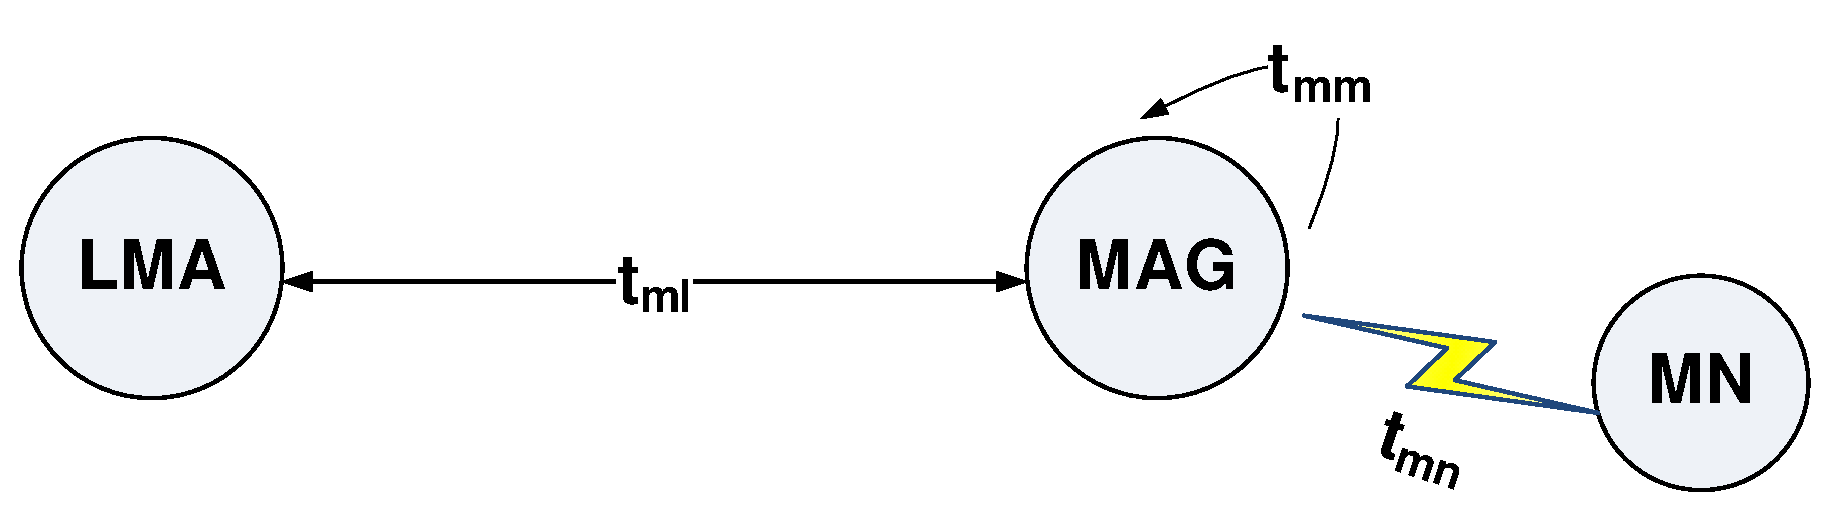
\includegraphics[width=0.50\textwidth]{./Part2/Chapter4/figures/c6_topology_analysis.eps} 
    \caption[Reference network topology for the  multicast service disruption time analysis.]{Reference network topology.}
     \label{fig:c6_topology_analysis}
  \end{center} 
\end{figure}

Fig.~\ref{fig:c6_topology_analysis} shows a reference topology for performance analysis. The delay factors consisting of total
delay are defined as follows:
\setlength \abovedisplayskip{-1pt}
\vspace{-0.1in}
\begin{itemize}
\itemsep 0.07em
\item $t_{mm}$: the delay between two MAGs.
\item $t_{ml}$: the delay between MAG and LMA.
\item $t_{mn}$: the delay between MAG and MN.
\item $t_{msa}$: the multicast service activation time.
\item $t_{qrd}$ the query response delay.
\end{itemize}

The service disruption time for multicast service is defined as a period when a multicast listener cannot receive the multicast packets. Thus, as can be seen in Fig.~\ref{fig:c6_handover}, it can be split into three main contributions (as stated in Chapter \ref{ch:performance_evaluation}): i) Layer 2 (L2) handover latency ($t_{L2}$); ii) Layer 3 (L3) handover duration ($t_{L3}$) caused by IP-related procedures. In PMIPv6, it includes the time for mobility management procedures (movement detection and location update procedures); and iii) The delay due to the multicast-related procedures, called $t_{M}(.)$.

Since in the proactive mode of M-LMA approach, it is not always feasible to the MN de-registers on the LMA by the previous MAG before attaching to the new one. Also, in the M-FPMIP approach, the under link radio access technology needs to support layer-2 triggers. Thus, in this section, the performance analysis will be done considering only the M-LMA (reactive-mode), the M-MLD and the M-CXT approaches. 

\begin{figure}[h!] 
 \begin{center} 
 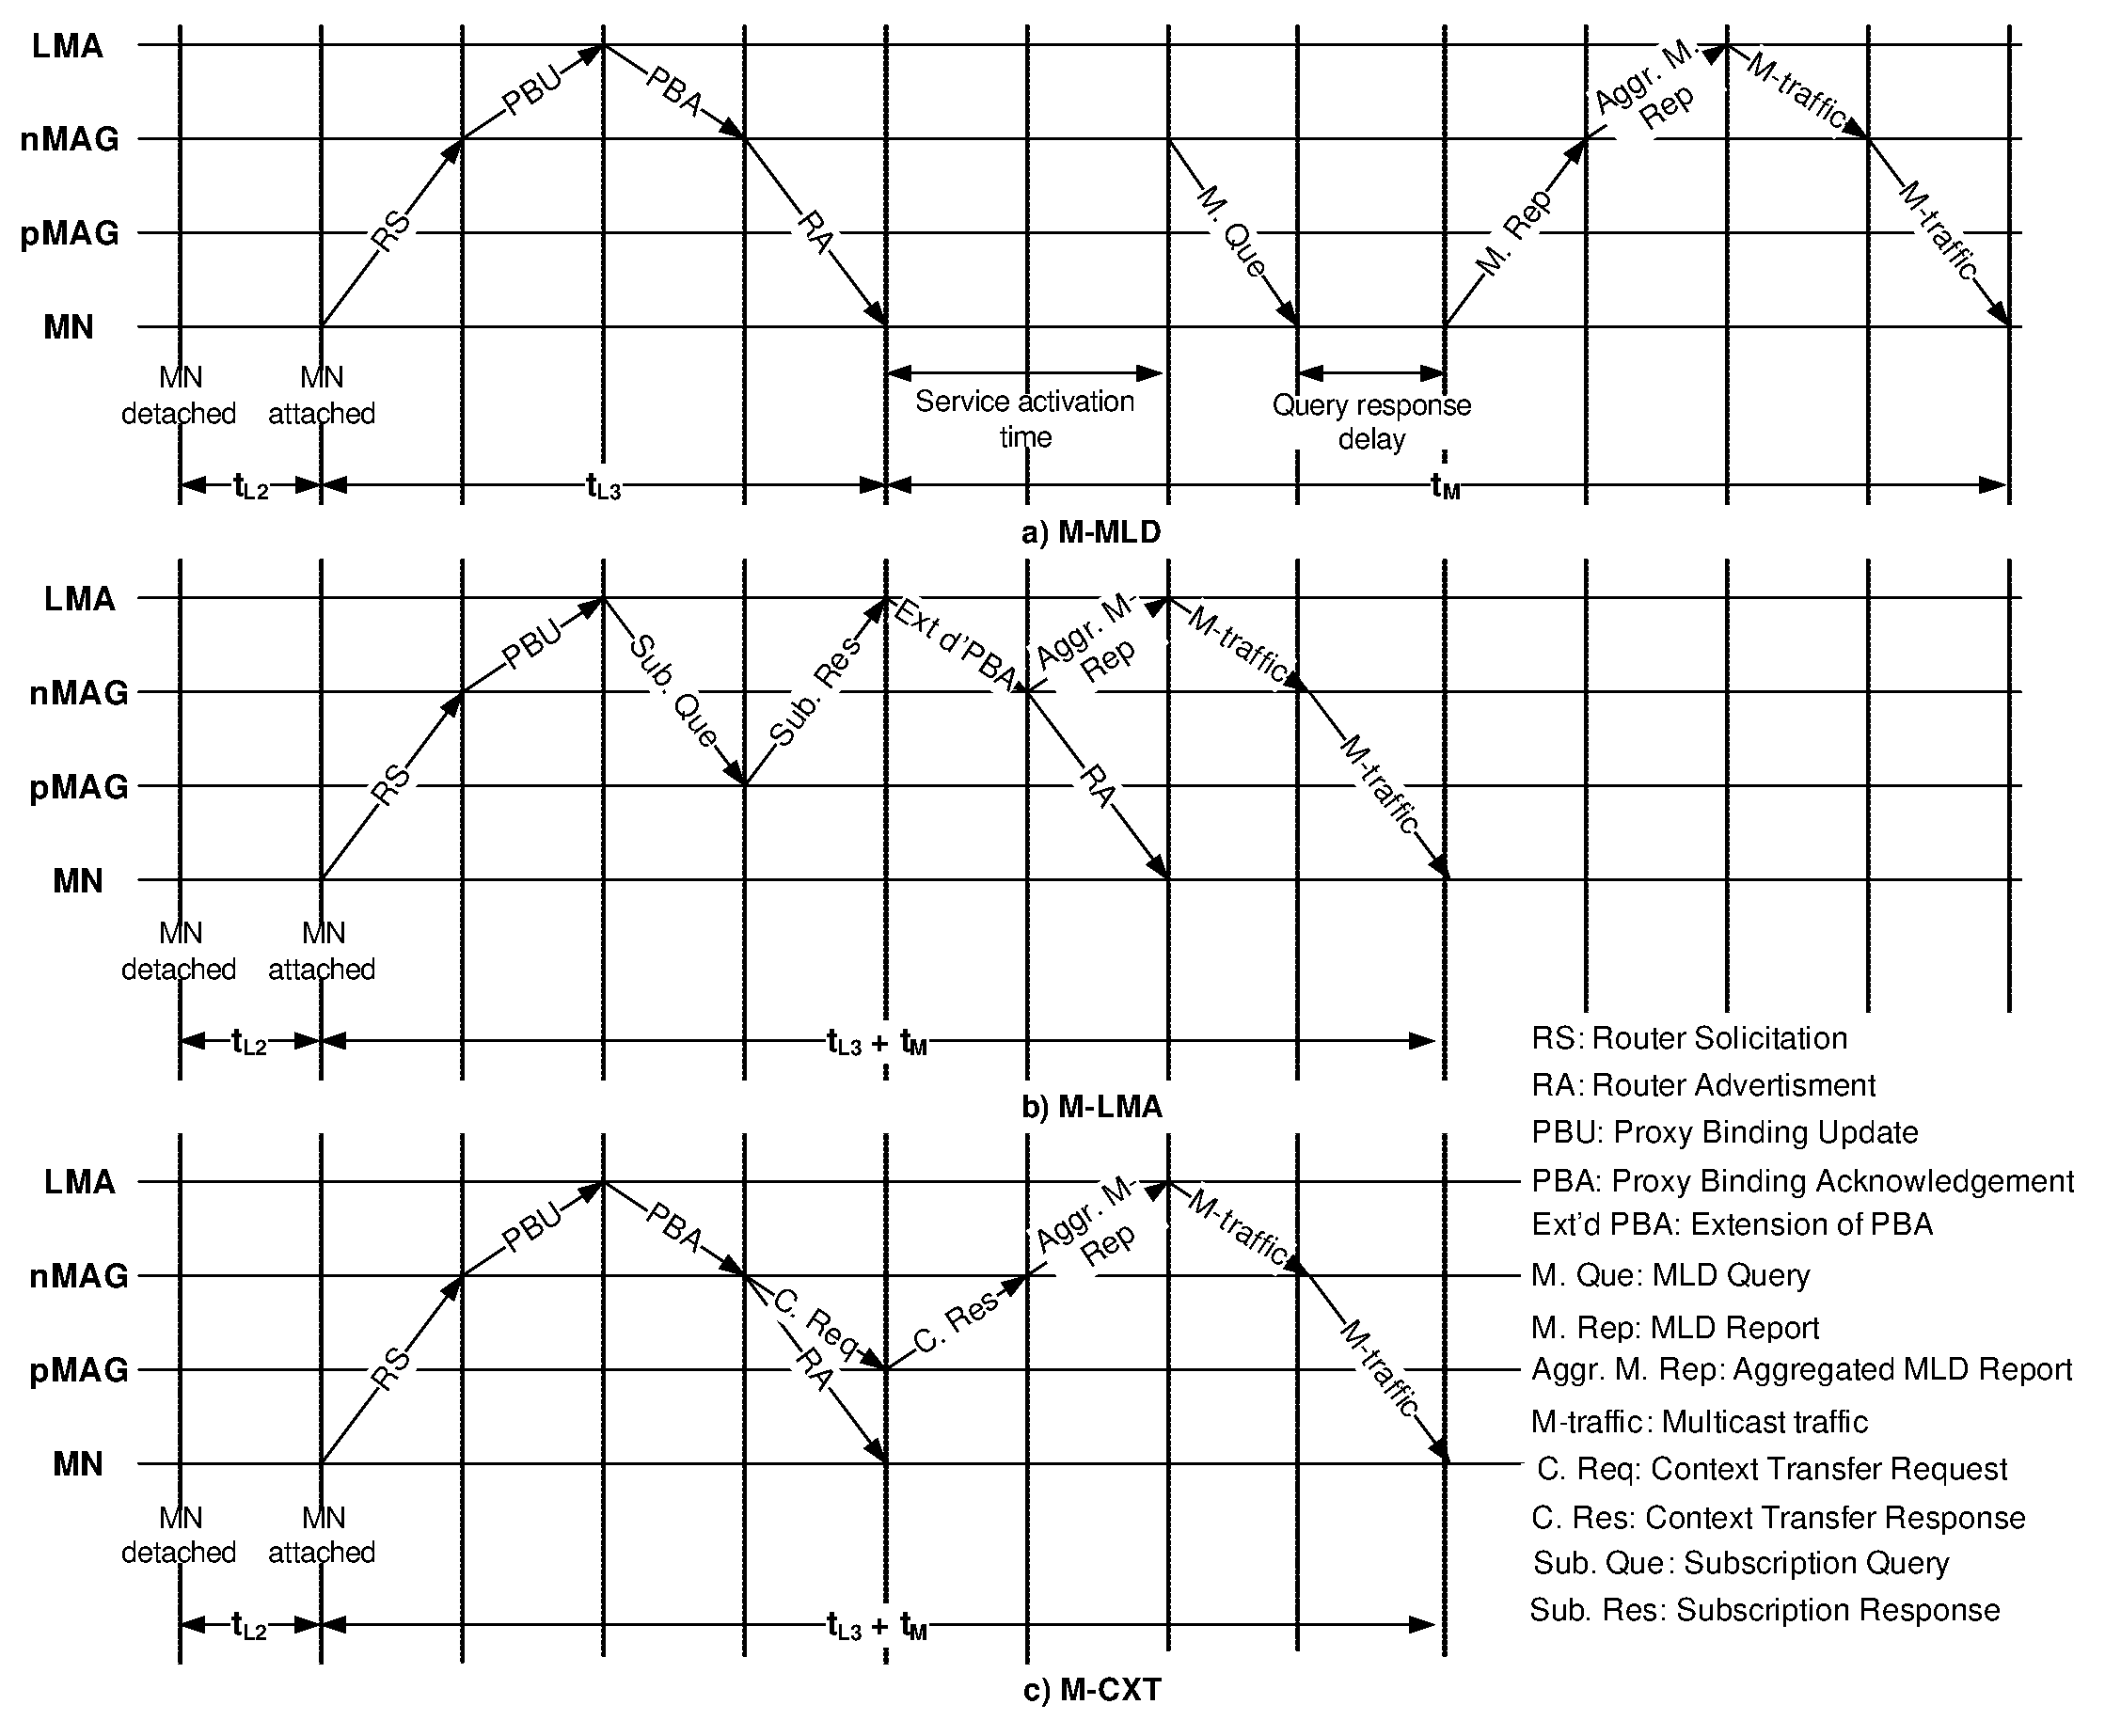
\includegraphics[width=0.85\textwidth]{./Part2/Chapter4/figures/c6_handover.eps} 
    \caption[Multicast-related signaling when a listener performs a handover inside a PMIPv6 domain.]{Multicast-related signaling for handover: (a) M-MLD, (b) M-LMA, (c) M-CXT.}
     \label{fig:c6_handover}
  \end{center} 
\end{figure}

Let $t_{X, Y}$ denote the delay between node X and node Y.  Then, the service disruption time is defined as \\
\begin{equation}
SD (.) = t_{L2} + t_{L3} + t_{M}(.),
\end{equation}
where $t_{L3}$ and $t_{M}(.)$ are given by\\
\begin{equation}
t_{L3} = 2t_{mn} + 2t_{ml}, 
\end{equation}
\begin{equation}
t_{M}(M-MLD) = t_{msa} + t_{qrd} + 3t_{mn} + 2t_{ml},
\end{equation}
\begin{equation}
t_{M}(M-LMA) = t_{mn} + 4t_{ml},
\end{equation}
\begin{equation}
t_{M}(M-CXT) = t_{mn} + 2t_{mm} +2t_{ml}.
\end{equation}

We suppose that MLD Queries are followed immediately the link-up event or the auto-configuration of IPv6 link-local address of an MN \cite{RFC_6224}. As a consequence, the multicast service activation time can be ignored ($t_{msa}$ = 0). As such, the total disruption time in the M-MLD approach is \\
\begin{equation}
SD(M-MLD) = t_{L2} + t_{qrd} + 5t_{mn} + 4t_{ml}.	
\label{eq:c6_total}
\end{equation}

In case of M-LMA approach, the service disruption is calculated as\\
\begin{equation}
SD(M-LMA) = t_{L2} + 2t_{mn} + 6t_{ml}. 	
\end{equation}

Using the multicast context transfer and the explicit tracking function, the context transfer function and layer 3 operations are executed in parallel as illustrated in Fig.~\ref{fig:c6_handover} (c). Consequently, the service disruption time in the M-CXT approach is calculated as follows\\
\begin{equation}
SD(M-CXT) = t_{L2} + 2t_{mn} + 2t_{mm} + 4t_{ml}. 	
\end{equation}

\section{Experimentation Setup and Scenarios Description} \label{section:testbed}
\begin{figure}[h!] 
 \begin{center} 
 \includegraphics[width=0.60\textwidth]{./Part2/Chapter4/figures/c6_testbed.eps} 
    \caption[PMIPv6 testbed for mobile multicast experimentation.]{Virtual PMIPv6 testbed.}
     \label{fig:c6_testbed}
  \end{center} 
\end{figure}

A reference topology for multicast support in a PMIPv6 domain is illustrated in Fig.~\ref{fig:c6_testbed}. The testbed - which consists of one LMA, three MAGs and two MNs, was developed based on the method described in Chapter \ref{ch:performance_evaluation}. For a quick reminder of this method, the testbed is a combination of virtual machines and wireless environment provided by the network simulator NS-3. The PMIPv6 entities (LMA, MAG) are the virtual machines while the access points (AP) and mobile nodes (MN0 and MN1) are NS-3 nodes. MN0 plays the role of a multicast source while MN1 plays the role of a multicast listener. Acting as a multicast listener, MN1 is subscribed to the multicast channel which is being broadcasted by the source. To deploy a PMIPv6 domain, the open source PMIPv6 implementation, named OAI PMIP \cite{oai_pmip}, is used. In OAI PMIPv6 implementation, the attachment/detachment phase for the MNs relies on SYSLOG \cite{syslog} message exchanged between Client (at the AP) and Server SYSLOG (at the MAG). Thus, the Client SYSLOG function is implemented in NS-3 and deployed at the APs. 

To enable the multicast support in a PMIPv6 domain, the MLD proxy function needs to be deployed at the MAG while the multicast routing function is provided at the LMA. There are two typical implementations of MLD proxy such as McProxy\footnote{McProxy - Multicast Proxy for IGMP/MLD, Homepage: http://mcproxy.realmv6.org/}, ECMH\footnote{ECMH - Easy Cast du Multi Hub, Homepage: http://unfix.org/projects/ecmh/}. Though the former is newer, it only supports MLDv1. That is why ECMH is selected. Yet, some functions need to be added into ECMH to support the multicast source mobility. On the other hand, the considered multicast routing protocols are PIM-SM/SSM \cite{PIM_SM}. There are two potential candidates providing PIM router functions: MRD6\footnote{MRD6, Homepage: http://fivebits.net/proj/mrd6/} and XORP\footnote{Xorp, Homepage: http://www.xorp.org/}. The first one is chosen because of its simplicity of deployment and configuration under UML. We also implemented the listener part of MLDv2 protocol under NS-3 to enable the multicast capability of NS-3 nodes.

\begin{figure}[h!] 
 \begin{center} 
 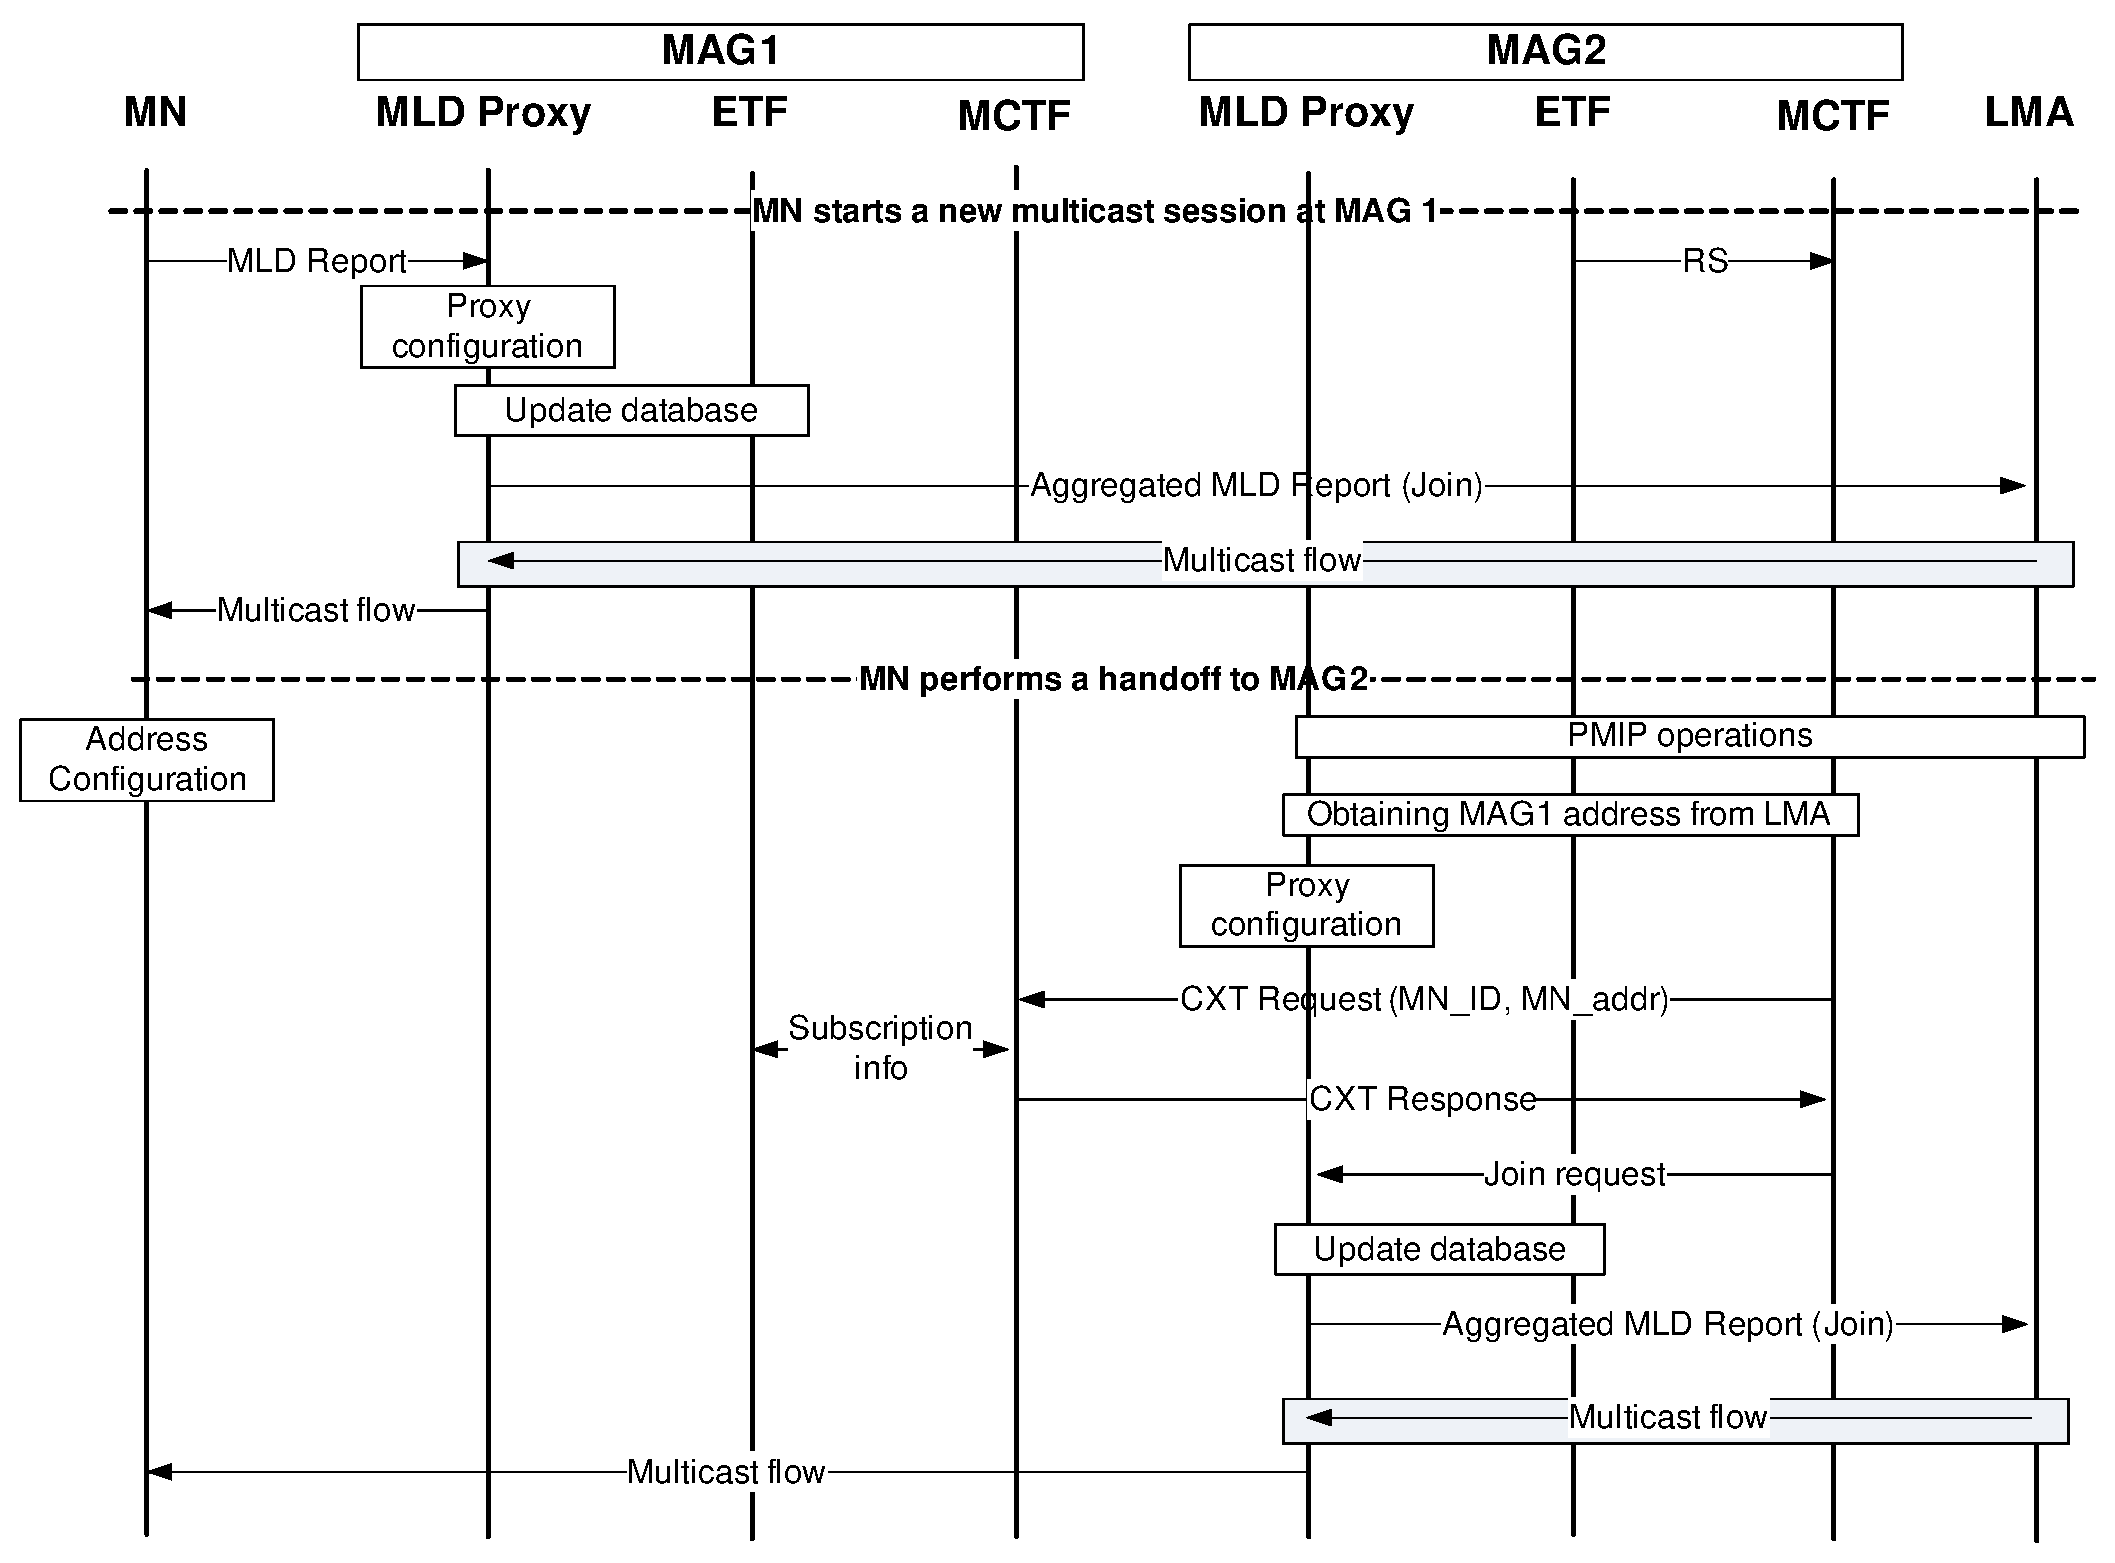
\includegraphics[width=0.750\textwidth]{./Part2/Chapter4/figures/c6_multicast_signaling.eps} 
    \caption[The interactions between components of the multicast mobility management module.]{Interaction between components of MUMO.}
     \label{fig:c6_multicast_signaling}
  \end{center} 
\end{figure}

In general, we implemented a multicast mobility management module (MUMO, in C/C++), which takes responsibility for all actions related to the multicast mobility as described in \cite{d4.2,d4.3} at the MAG. The structure of this module is briefly described as follows: i) The proxy function performs the operation of the MLD proxy (based on ECMH); ii) The explicit tracking function (ETF) maintains the per-host multicast membership state (can be considered as an extension to MLD proxy); and iii) The multicast context transfer function (MCTF) is responsible for the multicast context transfer exchanging between MAGs to reduce the service disruption time. The interaction between the different components of this module is illustrated in Fig.~\ref{fig:c6_multicast_signaling}. Note that the multicast context transfer function, which is developed as a separate sub-module, can be easily applied to the other solutions in PMIPv6 (e.g., direct-routing approach) as well as for the solutions in a DMM environment (see Chapter \ref{ch:multicast_dmm} for more details). 

From the fact that the service disruption time in M-CXT would be the same as in the M-LMA approach (as can be seen in Fig.~\ref{fig:c6_handover}), for a sake of simplicity we do not consider the M-LMA approach in our measurements. In other words, the experimentation will be conducted regarding only the M-MLD and the M-CXT approaches corresponding to two simulation scenarios as follows:
\begin{itemize}
\item Scenario 1: tuning the behavior of the MLD for routers (corresponding to the M-MLD approach). In this scenario, the regular behavior of MLD protocol takes place while the QRI is varied to measure the service disruption time. Upon receiving an MLD Query at the new link, the listener (MN1) replies by a regular MLD Report. Then, the nMAG sends an aggregated MLD Report to the LMA to join the multicast group on behalf of the listener. Thus, the multicast traffic originated from the source is routed from LMA to listener via the new tunnel LMA-nMAG. 
\item Scenario 2: using the multicast context transfer (corresponding to the M-CXT approach). When the multicast context transfer is used, by detecting the presence of a new listener, the multicast context transfer between nMAG and pMAG is executed, allowing nMAG to get the listener’s active multicast subscriptions. As an MLD proxy, nMAG joins the multicast group on behalf of the listener, and forwards the multicast packets to the listener.
\end{itemize}

To make sure that the experimental results reflect exactly the impact of the two strategies, the parameter QRI will be varied in both scenarios. According to \cite{MLDv2, tuning_MLD}, possible values of QRI using in the experimentation are 10, 5 and 2 seconds. Additionally, by now to simplify the experimentation, a simple mobility model is used: the listener moves between two MAGs with a fixed speed and a fixed direction. However, in the future, the mobility pattern will be applied to provide more flexible mobility of multicast listener. Also, the scenario in which many listeners are moving at the same time will be considered. To improve the credibility of the simulation results, we performed the experiment a large amount of times for each scenario. Based on the collected results, we calculate the average value and the standard deviation to improve the degree of confidence.

\section{Results and Discussions} \label{section:results}
\subsection{Results}
\paragraph{Numerical Results} In our analysis, $t_{L2}$, $t_{ml}$, $t_{mm}$ and $t_{mn}$ are assumed to be 50ms, 20ms, 10ms and 15ms, respectively, according to the literature \cite{d4.4}. Fig.~\ref{fig:c6_numerical_result} shows the numerical results. It is observed that the service disruption time in the M-MLD approach is definitely higher than that in the other approaches. On the other hand, the service disruption in case of M-CXT is a bit smaller than that in M-LMA (smaller is better). In other words, the M-CXT approach in general gives a similar performance in terms of service disruption as the M-LMA approach.
\begin{figure}[h!] 
 \begin{center} 
 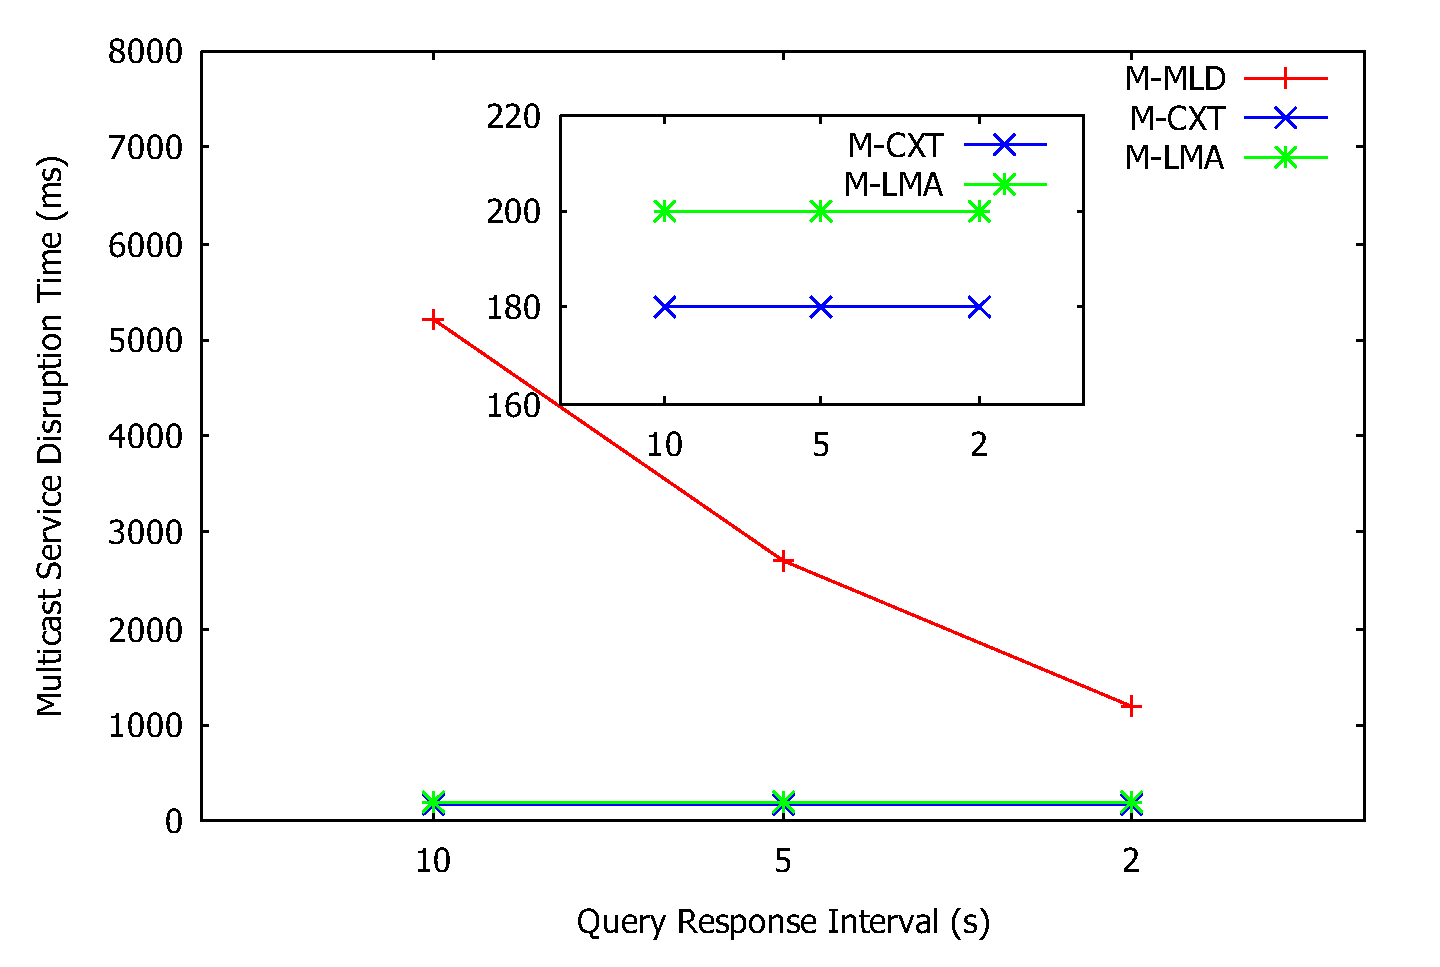
\includegraphics[width=0.60\textwidth]{./Part2/Chapter4/figures/c6_numerical_result.eps} 
    \caption[The multicast service disruption time: numerical results.]{Service disruption time: numerical results.}
     \label{fig:c6_numerical_result}
  \end{center} 
\end{figure}
\paragraph{Experimental Results} Fig.~\ref{fig:c6_simulation_result} describes the experimental results for the service disruption time in terms of mean ($<x>$) and standard deviation ($<\sigma_{x}>$). It appears clearly that the service disruption time in the M-MLD approach is absolutely higher than that in the M-CXT due to the value of $t_{qrd}$. As expected, the service disruption time in the former case decreases proportionally with the QRI, while almost keeping as a constant as the decreasing of QRI in the latter case. 
\begin{figure}[h!] 
 \begin{center} 
 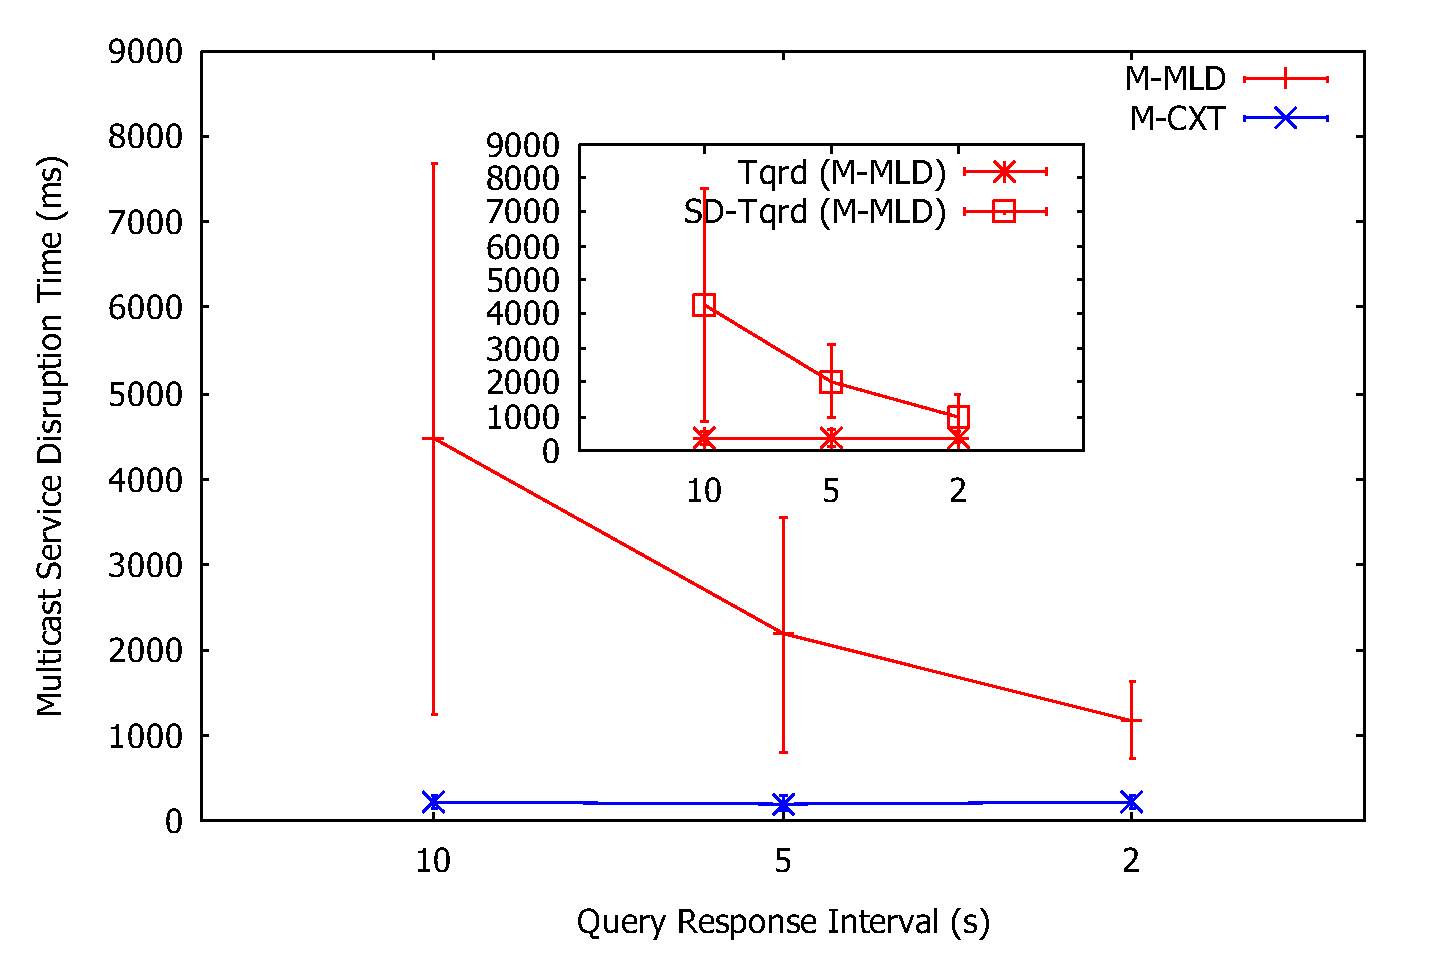
\includegraphics[width=0.60\textwidth]{./Part2/Chapter4/figures/c6_simulation_result.eps} 
    \caption[The multicast service disruption time: experimental results.]{Service disruption time: experimental results.}
     \label{fig:c6_simulation_result}
  \end{center} 
\end{figure}
The average value of service disruption time in the M-MLD is 1180ms ($\sigma$= 445.4ms) in the best case (when QRI is set to 2s), which still makes the impact of handover noticeable. If the multicast context transfer is used (M-CXT), in average, the service disruption time is around 220.53ms. Consequently, the handover impact on the quality of multicast stream is almost imperceptible. The variation of service disruption time in the M-MLD approach is clearly seen since it depends on several factors like scanning, association, authentication and $t_{qrd}$. Even $t_{qrd}$ can spread out over the large interval [0, QRI], $<t_{qrd}>$ is definitely higher than that of other delay types (L2 and L3). Hence, $t_{qrd}$ is the crucial factor in the service disruption time.
\begin{figure}[h!] 
 \begin{center} 
 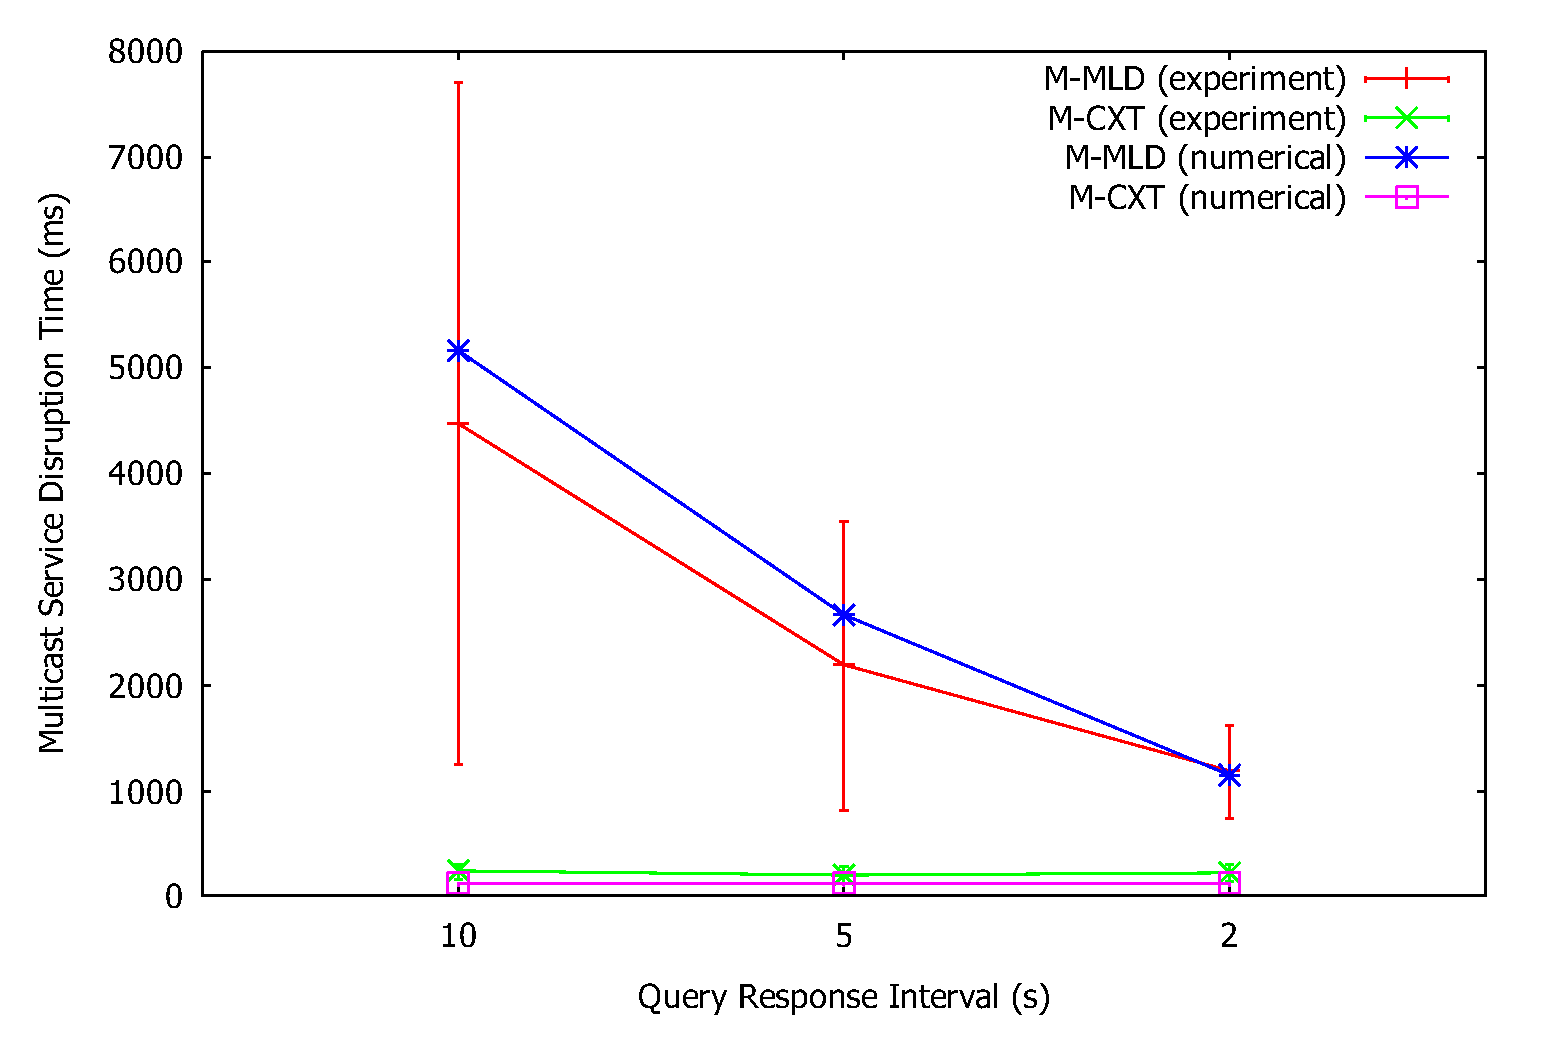
\includegraphics[width=0.60\textwidth]{./Part2/Chapter4/figures/c6_comparision.eps} 
    \caption[The multicast service disruption time: experimental vs. numerical results.]{Service disruption time: experimental vs. numerical results.}
     \label{fig:c6_comparision}
  \end{center} 
\end{figure}
\paragraph{Numerical vs. Experimental Results} Now the comparison between the numerical and the experimental results is investigated. For a fair comparison, we do not consider $t_{L2}$, since it depends on a specific wireless technology. Fig.~\ref{fig:c6_comparision} describes the numerical and experimental results. It is observed that the experimental results are, in general, in line with the theoretical analysis.
\subsection{Discussions}
\paragraph{Impact of QRI Reduction on the Wireless Link Condition}
If no multicast context transfer is used, the service disruption during handover can be clearly seen, even in the best case (QRI=2s). To minimize the handover effect, the value of the query response delay ($t_{qrd}$) needs to be reduced. It is done by decreasing the QRI. This reduction facilitates to achieve a seamless handover but makes the traffic more bursty, leading to the signaling overhead over the air interface. 

Following the MLDv2 protocol operation, after receiving an MLD query (periodical query or a query caused by a link-up event), the multicast listeners reply by an MLD Report at the interval selected randomly from the range [0, QRI]. As such, during the period [0, QRI] there are $n$ MLD Report messages generated on the link (where $n$ is the number of multicast nodes attached to MAG). The number of signaling messages is dramatically increased compared with those in case of the context transfer (only 2 messages are exchanged between MAGs via a wired link). 
The total air interface signaling overhead in the uplink direction is calculated as the size of MLD Report message multiplied by the number of MLD Report messages per second. Let $s$ denote the average size of MLD Report message, which is 96 bytes \cite{d4.3}. Thus, the total overhead is expressed as\\
\begin{equation}
OH = \frac{n \cdot s}{QRI}
\end{equation}

From the experimental results, $SD(M-CXT)$ in the worst case is 507.5ms. From Eq. (\ref{eq:c6_total}), to achieve a similar delay without any context transfer, $t_{qrd}$ must be less than or equal to a value of 352.4ms (when $t_{L2}$ = 0.1ms). It is done by setting QRI to a value of 352.4ms. It was also proven by the simulation results in which the mean and standard deviation of service disruption time are 465.43 and 70.3 ms, respectively. With this value of QRI, Fig.~\ref{fig:c6_mld} illustrates the air interface overhead. In more details, Fig. \ref{fig:c6_mld_n} shows the overhead as a function of the number of listeners attached to one MAG. As the number of listeners increases, the signaling overhead increases. For example, considering a typical PMIPv6 deployment in which a MAG severs approximately 5000 MNs \cite{RFC_6224}, the signaling overhead is 10896 kbits/s ($\approx 10.8 Mbit/s$). It may cause a negative impact to the wireless network since the wireless link is a typically bandwidth limited. 
Fig~.\ref{fig:c6_mld_qri} shows the signaling overhead when the value of QRI is varied over a range [100, 2000]ms. The overhead decreases when QRI increases. When QRI is small, the signaling overhead causes a noticeable impact to the wireless link. Thus, it is obvious that reducing the service disruption by using QRI should be carefully investigated at a cost of high signaling overhead and increase of power consumption at the mobile node. 

\begin{figure}[h!]
\centering
\subfloat[]{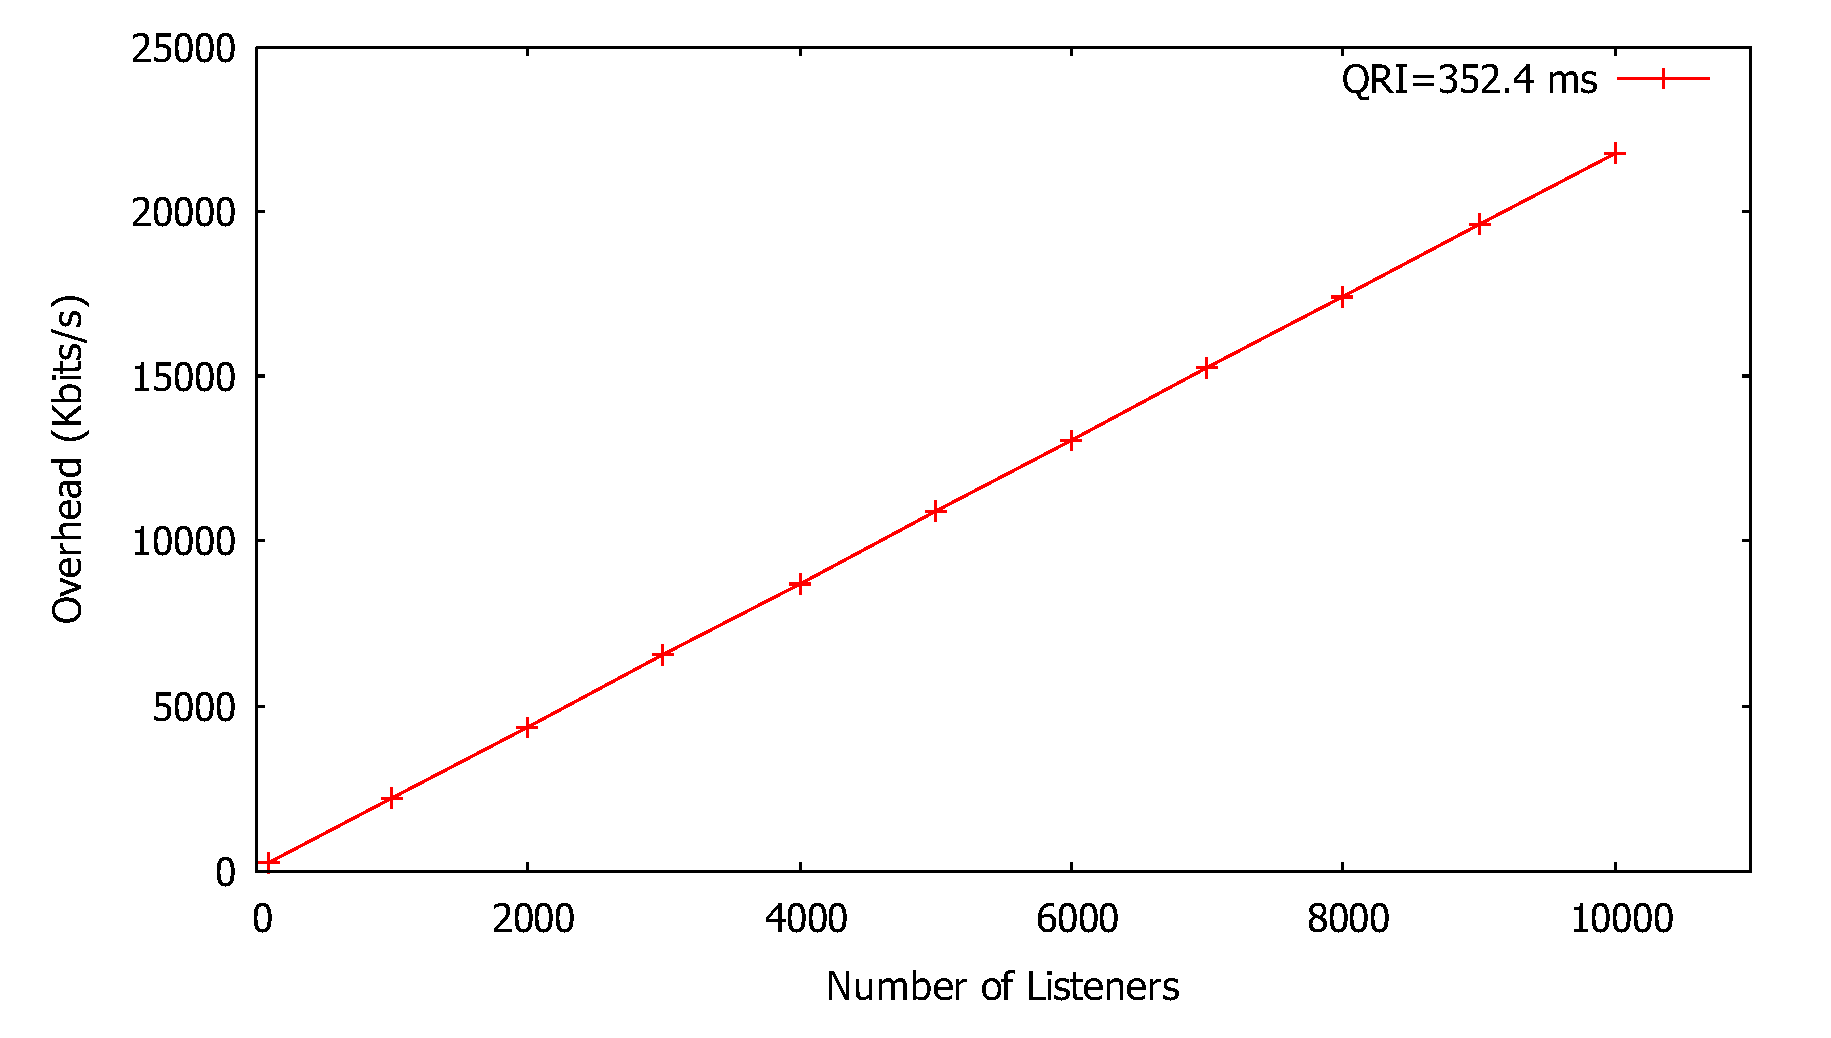
\includegraphics[width=0.47\textwidth]{./Part2/Chapter4/figures/c6_mld_n.eps} \label{fig:c6_mld_n}}\,\,\,\,\,\,
\subfloat[]{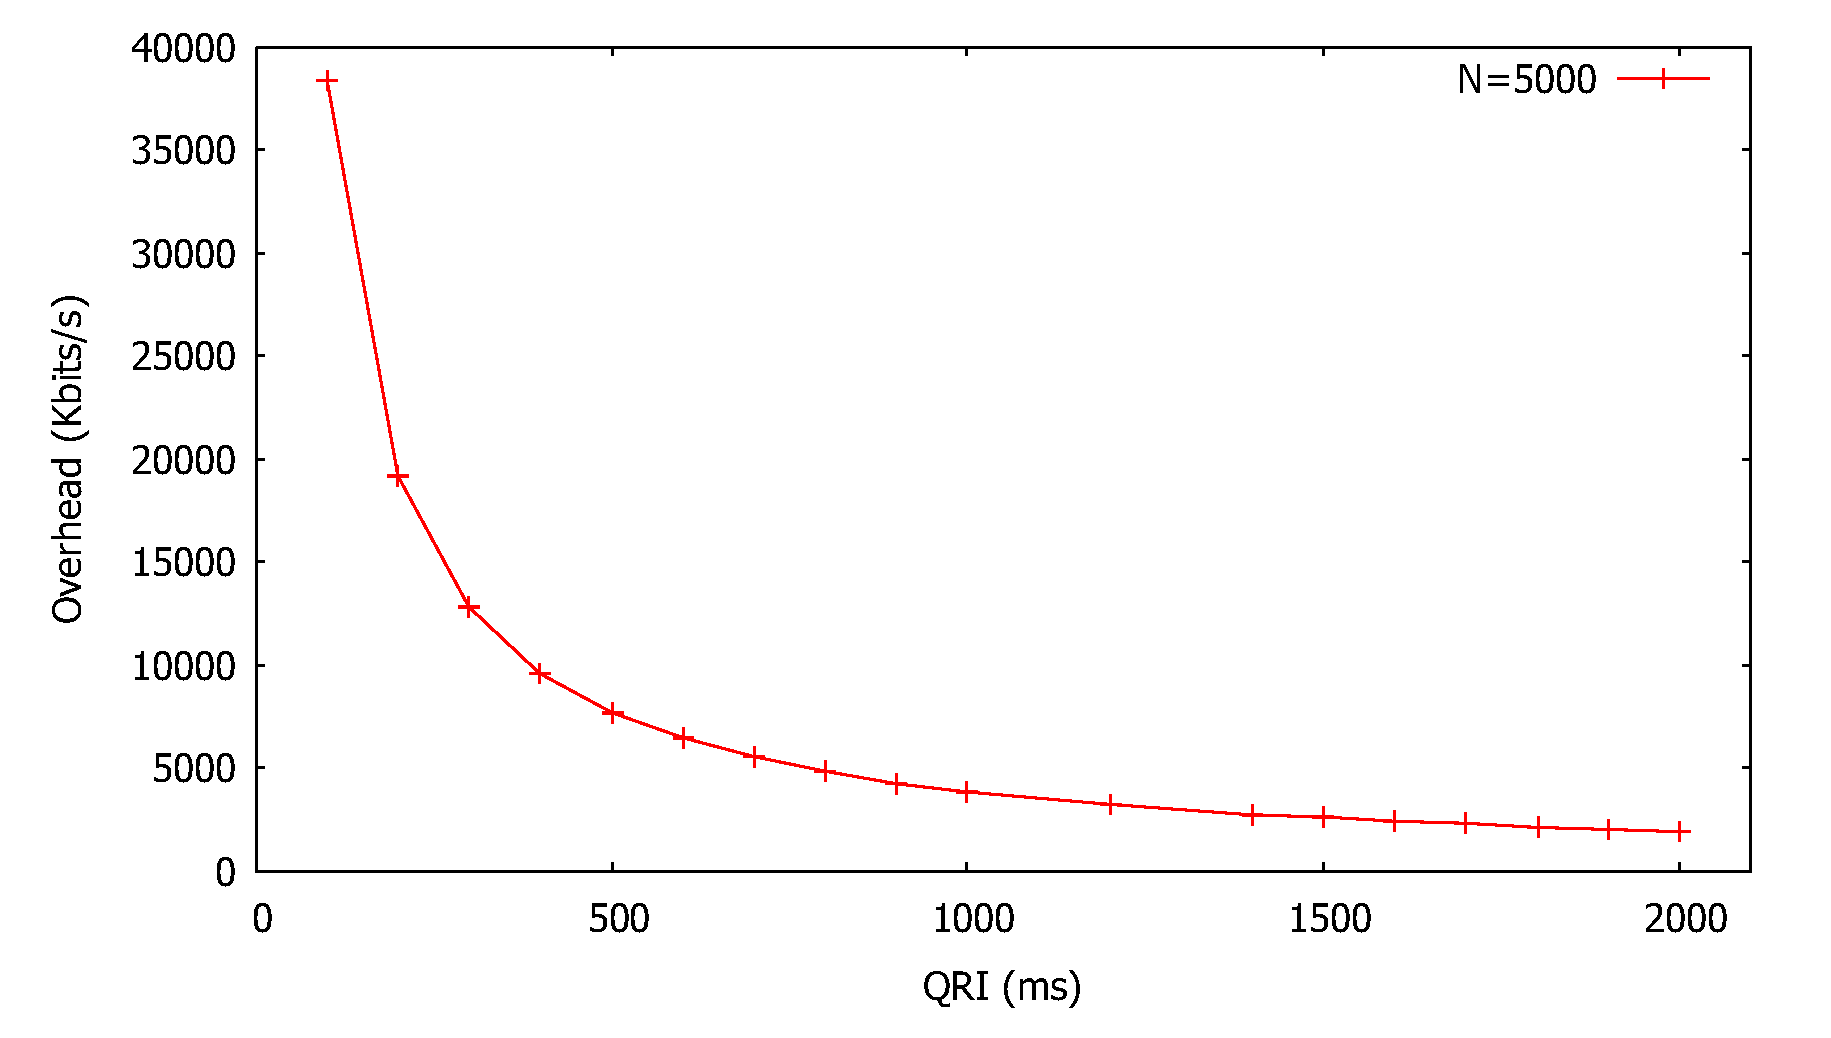
\includegraphics[width=0.47\textwidth]{./Part2/Chapter4/figures/c6_mld_qri.eps}\label{fig:c6_mld_qri}}
\caption[Multicast-related signaling overhead over the air interface.]{Air Interface signaling overhead: (a) as a function of number of listeners (n), (b) as a function of QRI.}
\label{fig:c6_mld}
\end{figure}

\paragraph{Waste of Resource (Leave Latency) Issue}
Due to mobility, the listener moves from the pMAG to the nMAG without explicitly sending an MLD message to leave the multicast group at the pMAG. As a result, if the listener is the last member of this group, the pMAG still continues forwarding this flow until it updates the membership information. In more details, according to \cite{MLDv2} the MLD proxy at pMAG has to wait to the source timer expires, then sends a source specific query and waits for a report during the time specified by the value of Last Listener Query Timer (LLQT) (during LLQT time, the pMAG should send Last Listener Query Count (LLQC) - 1 retransmissions of the query). The source timer at the beginning is set to the value of the Multicast Address Listening Interval (MALI). As a result, the total time needed for the pMAG to recognize that the last member has left its subnet is calculated as \\
\begin{equation}
LL = MALI - T_{leave} + LLQT,
\end{equation}
where 
\begin{equation}
MALI = RV \cdot QI + QRI,
\end{equation}
\begin{equation}
LLQT=  LLQI \cdot LLQC,
\end{equation}
where LLQI is Last Listener Query Interval and RV is the Robustness Variable. 
$T_{leave}$ is the interval time between the last source timer update and the moment where the listener leaves the pMAG. Thus, in average\\
\begin{equation}
T_{leave} = \dfrac{QI+QRI}{2}
\end{equation}

Without the explicit tracking function, the default value of RV, QRI, QI, LLQI and LLQC is 2, 10s, 125s, 1s and 2, respectively.  While in case of explicit tracking function, the value of RV can be set to 1 or 2 depending on the link condition \cite{tuning_MLD}. Also, QRI may be set to 5, 10, and 20s. Thus, in the normal case, the leave latency is 194.5s, while in case of explicit tracking is 191s (in the best case, where RV and QRI are set to 1s and 5s, respectively). During this period, the pMAG continues forwarding the multicast traffic even though no listener is interested in this flow, leading to a significant waste of resource. Even with the explicit tracking function, the leave latency is slightly reduced. Taking benefit of the context transfer function, the nMAG can request the pMAG to stop forwarding the multicast flow by means of CXT Request message (see Fig.~\ref{fig:c6_multicast_signaling}). Thanks to this mechanism, in our experiment the leave latency is 105.6ms (standard deviation = 45.2). Thus, the leave latency is negligible.   

\section{Conclusion} \label{section:conclusion}
This chapter focused on the effect of using the multicast context transfer and tuning the behavior of the IGMP/MLD for routers on handover performance of multicast listener mobility. The numerical and experimental results showed that through the utilization of multicast context transfer, the service disruption time could be reduced significantly without increasing the multicast-related signaling. We also observed that by tuning the behavior of the IGMP/MLD for routers, we could achieve a similar result, but make a noticeable multicast-related signaling increase. Thus, the impact of the multicast-related signaling on the wireless link by the number of listeners and the value of QRI was studied. In addition, the solution based on the multicast context transfer helps minimizing the handover latency. This chapter also presented an enhanced version of the testbed described in Chapter \ref{ch:performance_evaluation} by introducing the multicast mobility support. We deployed a real implementation for the multicast context transfer and explicit tracking functions on our testbed. This implementation then can be directly applied in a real testbed. In more details, in the Medieval project, the real multicast testbed \cite{d4.3, d4.4} has been deployed to validate the effective of multicast context transfer for PBS consumers over a DMM environment.   
